\chapter{Implementation}

All aspects of \Backpack{}, as described in this thesis,
have been implemented in GHC 8.2 and cabal-install 2.0.  In this
chapter, we describe some nontrivial aspects of our implementation.

\section{Opaque unit identifiers}

\Uid{}s are abstract syntax trees which are passed aroudn throughout
the compiler.  The downside is that instantiated \uid{}s
can be quite large (in part because \cid{}s allocated by the
package manager can be quite large, as they must record information
about how dependency resolution was performed for the library),
wasting memory in the compiler.

Fortunately, in some cases, the structure of a \uid{} is not necessary;
for example, when a unit identifier has no module holes, it is
invariant under substitution.  A useful optimization in this case
is to represent the structure opaquely with a \emph{definite unit
identifiers}.  The abstract structure of a \uid{} now looks like this:

\[
\begin{array}{rcll}
  \mathbb{P} &&& \text{Definite \uid{}} \\
  \UP &::=& \icid{\Up}{S} & \text{\Uid} \\
      & | & \mathbb{P} \\
\end{array}
\]

\noindent
Notice that definite \uid{}s occur recursively: the intent is that a
definite \uid{} be allocated for a library when it is fully instantiated
and compiled.  Thus, a definite \uid{} always corresponds to a \uid{}
whose module substitution refers all to definite \uid{}s (since those
libraries had to be compiled first, before this one could be compiled!)
When compiling a fully instantiated library, the only \uid{}s which the
compiler needs to interact with are definite \uid{}s, meaning that we
only have to pay the cost of a full \uid{} when typechecking uninstantiated
libraries.

Definite \uid{}s are purely an implementation mechanism; if a definite
\uid{} and a normal \uid{} are compared, the comparison must be done
up to unfoldings of the definite \uid{}, as seen below (definite \uid{}s
highlighted in blue):

\begin{figure}[H]
\center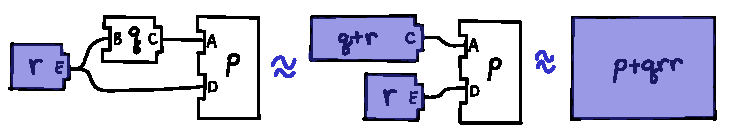
\includegraphics{figures/unit-identifier-improvement.pdf}
\end{figure}

\section{No symbol tables}

Compilers usually have one or more data structures known as
\emph{symbol tables}, which are mappings from symbols to information
about the symbol: abstractly, the symbol table is represented by
the \emph{context} in which typechecking takes place.
In contrast, GHC avoids symbol tables:  instead, a
symbol \emph{contains} all information about itself, forming an
immutable \emph{cyclic data structure} of all symbols
known to GHC\@.  For example, here are
some data types for the graph representation from GHC (simplified
and abbreviated):

\begin{lstlisting}
    data Type  = TyConApp TyCon [Type]  | ...
    data TyCon = SynonymTyCon Name Type | ...
    data ModDetails = ModDetails [TyCon] ...
\end{lstlisting}
%
A type may be an application of a type constructor to some arguments, in which
case it contains a type constructor \verb|TyCon|.  A type constructor
can be a type synonym, in which case it contains the type it expands
to.  A module \verb|ModDetails| consists of a list of type constructors
and other entities that are defined in it.  The ``graph'' is the graph of
heap objects which represent these data types.

This graph is very convenient to work with in a purely functional
language like Haskell, since queries can be answered by a direct field
access rather than a lookup in a symbol table.  For example, type
equality can be defined as a pure function \verb|Type -> Type -> Bool|
even in the presence of type synonyms, since the \verb|SynonymTyCon|
always carries along the expanded version of the synonym to compare
against.

On disk, GHC doesn't store an infinite type; instead, its
interface representation closely resembles the semantic objects
we described in Section~\ref{sec:semantic-objects}:

\begin{lstlisting}
    data IfaceType = IfaceTyConApp Name [IfaceType] | ...
    data IfaceDecl = IfaceSynonym OccName IfaceType | ...
    data ModIface = ModIface [IfaceDecl] ...
\end{lstlisting}

\noindent
Unlike the graph representation, the type constructor application
doesn't embed the definition of the type constructor---instead,
it records only a \verb|Name| reference to the constructor. To find out
more information about the type constructor, you would have to lookup
the \verb|IfaceDecl| from the appropriate symbol table; e.g., a module
local declaration would be found in the \verb|IfaceDecl| list in
\verb|ModIface|.

GHC uses a technique called ``tying the knot''
to construct the graph representation from the interface
representation: any time we encounter a \verb|Name|, GHC instead
allocates a thunk to lookup the appropriate declaration later,
once all of the entities have been added to the environment.

\paragraph{Consequences for \Backpack{}}
In Section~\ref{sec:overview-compiler}, we informally described
types as graphs, with original names pointing to the corresponding
declaration.  In fact, this is an accurate representation of how
these operations are implemented in GHC\@!

One downside of the immutable graph representation is that it is
difficult to modify after the fact: in general, the only way to update
it is to rebuild the graph from scratch.  Modifications of this kind
frequently occur in \Backpack{}: for example, applying a name
substitution will change how the graph is wired.

To handle this, our implementation does most operations in two
phases:

\begin{itemize}
    \item We first perform any operations which would
    mutate the graph on the \emph{interface representation}.
    These operations includes both module and name substitutions, as well
    as signature merging.
    \item Then, we generate the \emph{graph representation} from
    the resulting interface representation, and then perform any
    operations which require consulting the context.  These
    operations include subtyping, which test equality on types
    and require the context.
\end{itemize}
%
Our typechecking rules are staged so that once we have generated the
graph representation, we don't need to regenerate it in the future.

\section{Interaction with type inference}

\Red{Note about inaccessibility}
